\section{Zusammenfassung und Diskussion}

Durch die Bestrahlung stabiler Isotope mit langsamen (thermischen) Neutronen, welche von den Kernen der Isotope eingefangen werden, ist es möglich, radioaktiver Quellen herzustellen. Dieser Prozess, die sogenannte Aktivierung, wurde in Versuch 252 untersucht. Hierzu betrachteten wir sowohl Silber- als auch Indiumisotope. Aus den stabilen Silberisotopen \isot{107}{Ag} und \isot{109}{Ag} werden durch den einfach von Neutronen die radioaktiven Isotope \isot{108}{Ag} und \isot{110}{Ag}. Aus dem stabilen Indiumisotop \isot{115}{In} werden durch die Aktivierung die radioaktiven Isomere \isot{116}{In} und \isot{116m}{In} erzeugt. 

Für den Versuch nahmen wir die Zahl der Zerfälle für das Silber in Intervallen von 10 Sekunden über 40 Messungen und für das Indium in Intervallen von 120 Sekunden über 25 Messungen mit einem Geiger-Müller-Zählrohr auf. Die Zahl der Zerfälle pro Sekunde, genannt Aktivität, folgt, nach der Aktivierung der Isotope, dem negativ exponentiellen Abfall des Zerfallsgesetzes. Ein solches Modell passten wir an die aufgezeichneten Daten an, um primär die Zerfallskonstante $\lambda$ zu bestimmen.

Betrachten wir zunächst die Güte des Fits an die Aktivität des Silbers. Der $\chisq$ Wert von $37.56$ ist etwas hoch, unter Berücksichtigung der Freiheitsgrade mit einem reduzierten $\chisq$ von etwa $1.04$ liegen wir allerdings im optimalen Bereich. Die Fitwahrscheinlichkeit von $40\%$ ist mit einem Wert um $50\%$ sehr gut und deutet darauf hin, dass das Modell die Messdaten gut beschreibt.

Für den Fit an die Aktivität des Indiums erhalten wir einen etwas niedrigeren $\chisq$ Wert von etwa $17.7$. Mit $0.84$ ist der reduzierte $\chisq$ Wert zwar etwas weiter unter dem optimalen Wert von $1$. Dies kann bedeuten, dass das Modell Unsicherheiten in den Messdaten etwas überschätzt. Die sehr gute Fitwahrscheinlichkeit von $67.0\%$, zeigt aber, ebenso wie die anderen beiden Werte, dass das Modell sehr gut zu den Daten passt.

Aus den durch die Fits ermittelten Zerfallskonstanten berechneten wir in der Auswertung die Halbwertszeiten der Isotope zu
\renewcommand{\arraystretch}{1.5}
\begin{table}[H]
    \centering
    \begin{tabular}{c|c}
        Isotop & Halbwertszeit\\\hline
        \isot{110}{Ag} & $(19.3 \pm 1.7)\,\si{\second}$\\
        \isot{108}{Ag} & $(105 \pm 9)\,\si{\second}$\\\hline
        \isot{116}{In} & $(53.1 \pm 2.2)\,\si{\minute}$\\
    \end{tabular}
\end{table}
\renewcommand{\arraystretch}{1}

Dies Werte möchten wir nun mit den Literaturwerten aus der Nuklidkarte \abbref{plot:nuklidkarte} vergleichen. Für die Halbwertszeit von \isot{108}{Ag} sind hier $2.41\si{\minute}$ angegeben, dies entspricht einer Abweichung von $4.4\sigma$ vom von uns berechneten Wert. Die angegebene Halbwertszeit von $24.6\si{\second}$ für \isot{110}{Ag} weicht um $3.2\sigma$ von dem von uns berechneten Wert ab.

Mit einer Abweichung von gerade einmal $0.4\sigma$ ist unser berechneter Wert der Halbwertszeit des Indiums sehr nah am Literaturwert von $54 \si{\minute}$ aus der Nuklidkarte.

\begin{figure}[H]
    \centering
    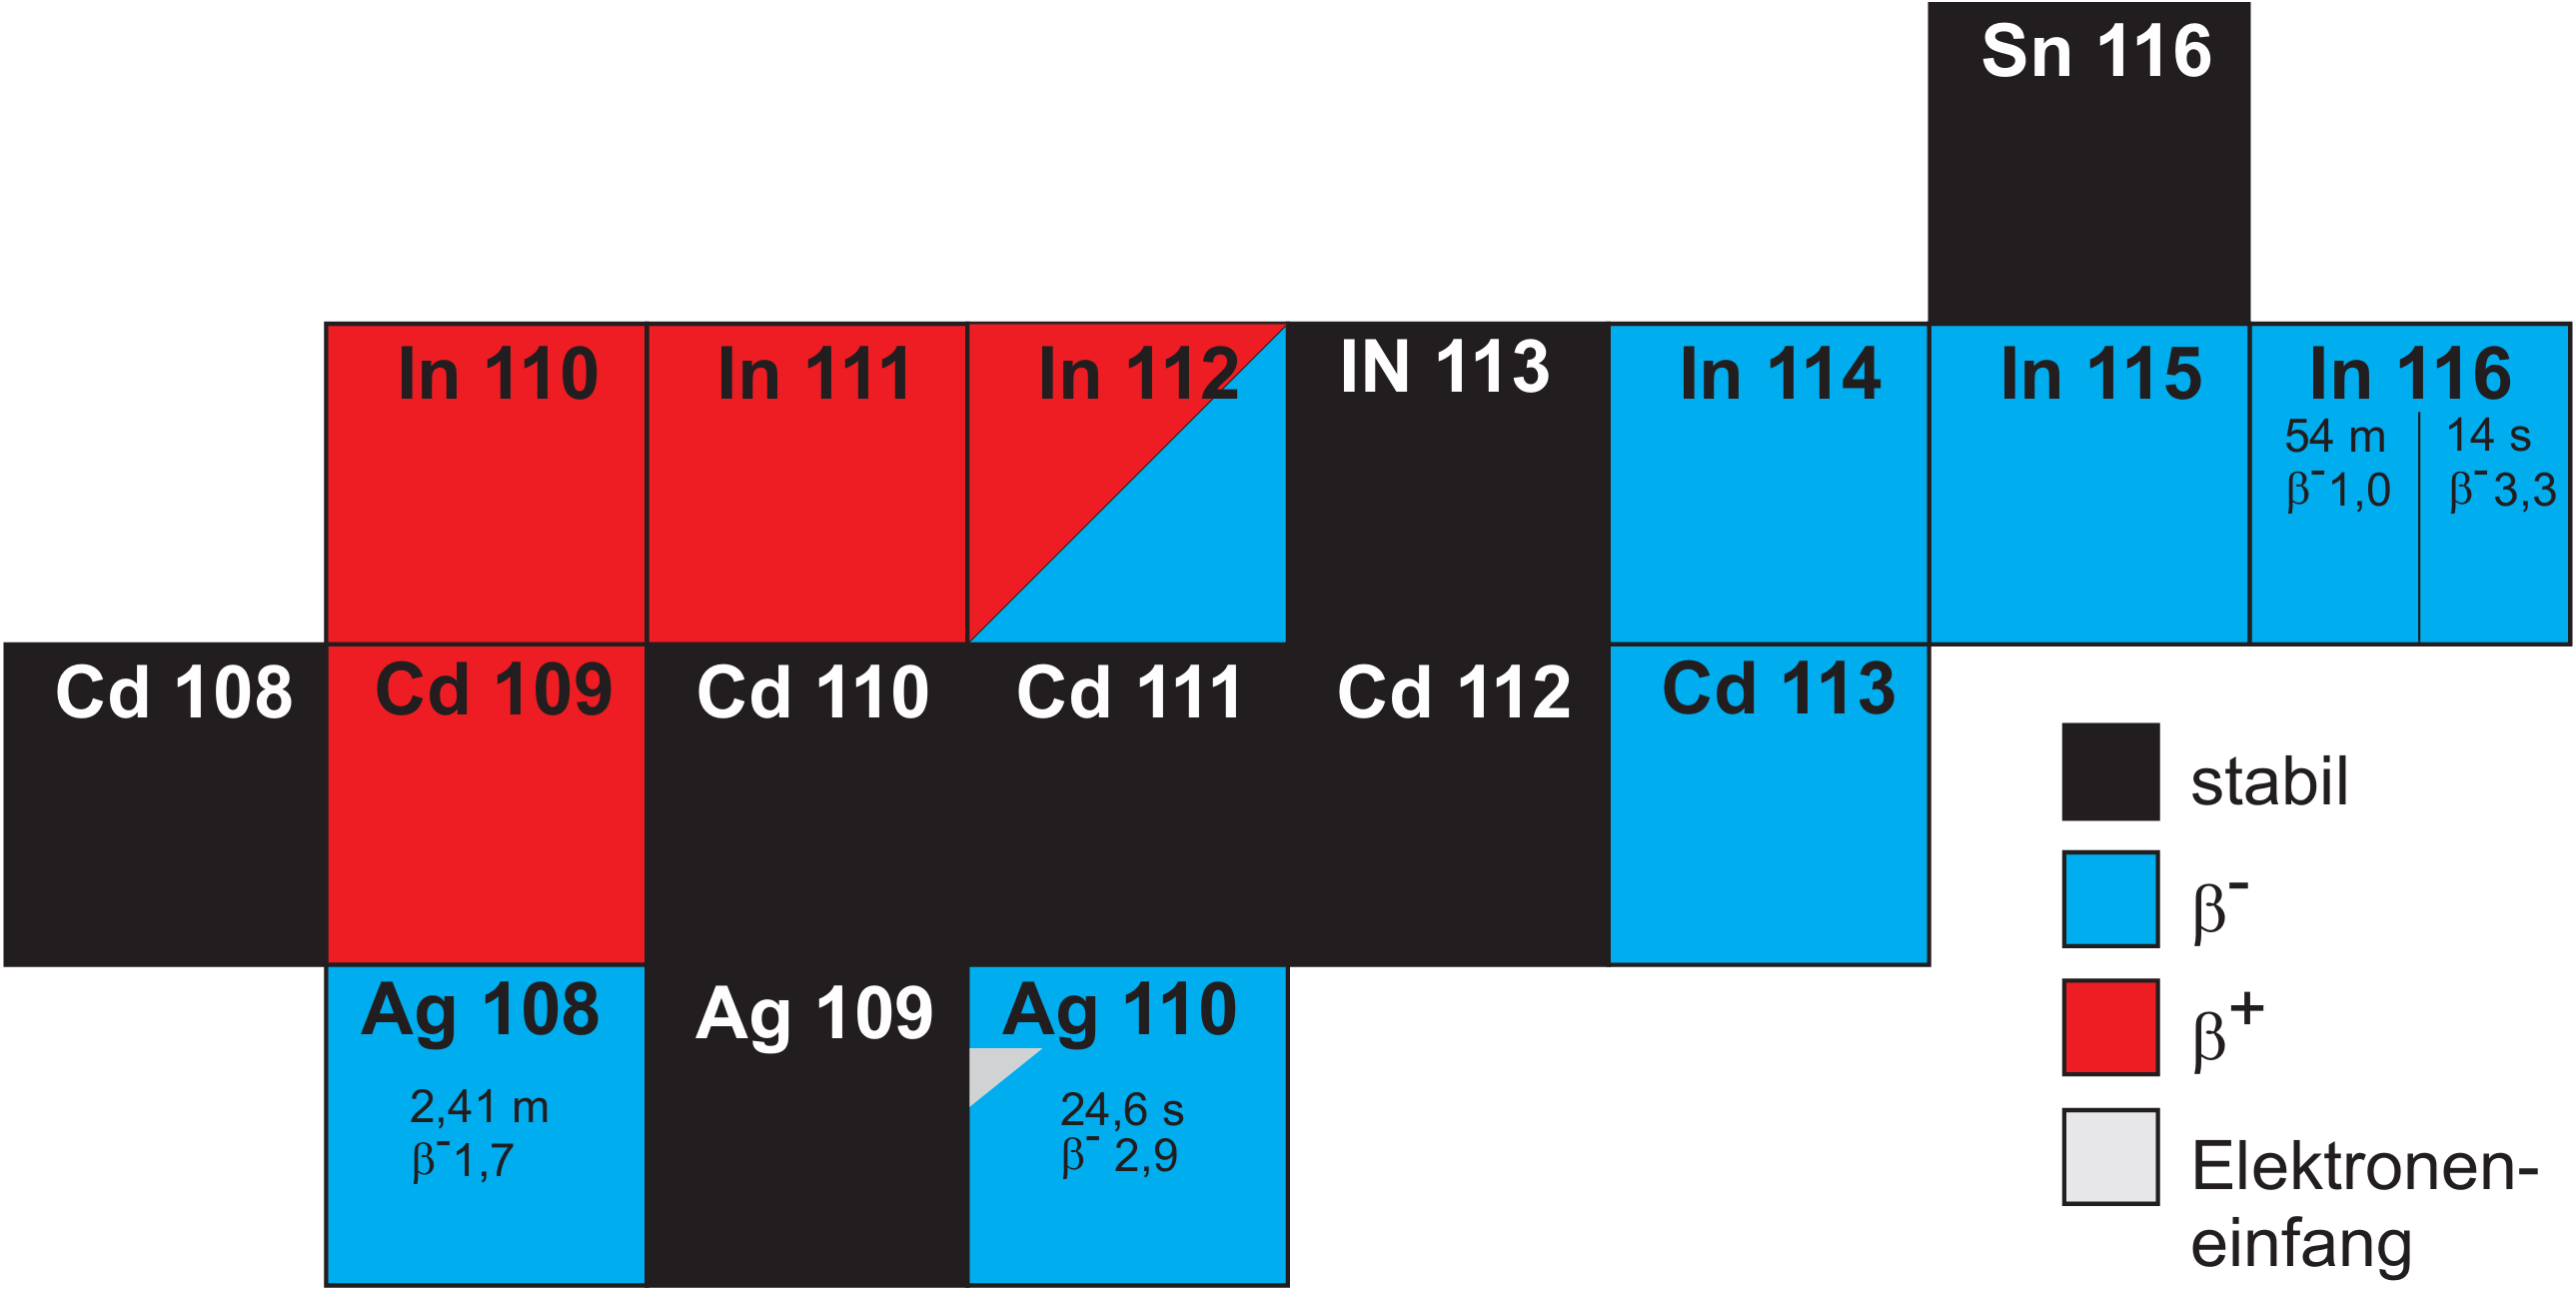
\includegraphics[width=.85\textwidth]{files/nuklidkarte.png}
    \caption{Ausschnitt der Nuklidkarte}
    \label{plot:nuklidkarte}
\end{figure}

Ein Großteil der Abweichungen wird hierbei vermutlich aus den Fits entspringen. Hierzu zählt zum einen die Abschätzung des Untergrundes. Bereits \abbref{plot:untergrund} zeigt, dass die Untergrundzählrate stark rauscht. In die Fits beziehen wir allerdings nur dessen Mittelwert als Konstante mit ein. Zwar betrachten wir noch gesondert die Auswirkungen der Fehler des Mittelwertes, trotzdem werden feinere Auswirkungen größtenteils unterschätzt.\newline\noindent
Im Fit der Aktivität des aktivierten Silbers könnte die gleichzeitige Betrachtung zweier zerfallenden Isotope Auswirkungen auf die Genauigkeit haben. Zwar lassen sich diese im Fitmodell mathematisch getrennt darstellen, in Realität kann es aber sein, dass hier dennoch Interaktionen und Überlagerungen stattfinden, welche vom Fitmodell nicht berücksichtigt werden. Betrachten wie die Daten des Indiumzerfalls, so fällt auf, dass der allererste Messpunkt deutlich über der angepassten Funktion liegt.\newline\noindent
Wie in der Einleitung erklärt, entstehen bei der Aktivierung des Indium-115 Isotops die Isomere \isot{116}{In} und \isot{116m}{In}. Hierbei hat \isot{116m}{In} die Halbwertszeit von etwa $54 \unit{m}$, während sie bei \isot{116}{In} lediglich etwa $14\unit{s}$ beträgt. Was wir als Abweichung im ersten Messpunkt sehen ist also der Zerfall des \isot{116}{In}, welcher sich kurz mit dem des \isot{116m}{In} Isotop überlagert. Trotz dieser kleinen Unreinheit in den Daten sehen kommen wir bei der Bestimmung der Halbwertszeit von \isot{116m}{In} auf ein sehr gutes Ergebnis.